\documentclass[tikz,border=5pt]{standalone}
\usepackage[utf8]{inputenc}
\usepackage[T1]{fontenc}
\usepackage{lmodern,amsmath,amssymb}
\usepackage[american]{circuitikz}
\usepackage{pgfplots}
\pgfplotsset{compat=1.18}
\usetikzlibrary{circuits.logic.US,positioning,calc,arrows.meta,patterns,shapes.geometric}
\definecolor{Primary}{HTML}{1F77B4}
\begin{document}
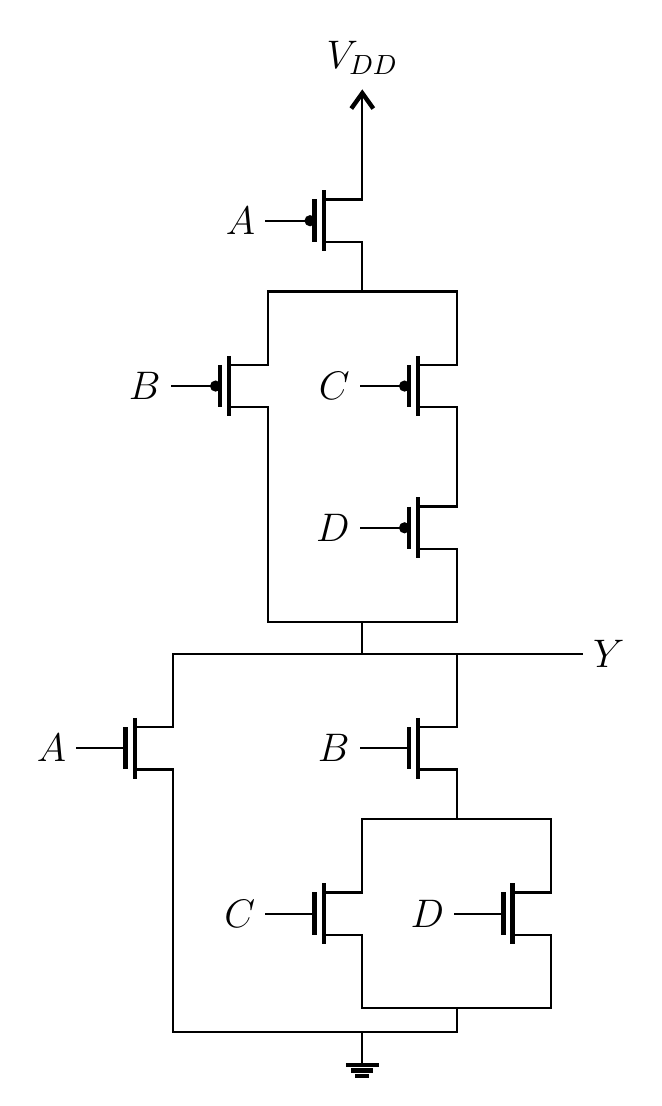
\begin{tikzpicture}[thick,font=\Large]\node[pmos](m33)at(0,5.5){};\draw(0,6.4)--(m33.S)(m33.D)--(0,4.6000000000000005);\draw(m33.G)--++(-.25,0)node[left]{$A$};\draw(0,4.6000000000000005)--(-1.2,4.6000000000000005)--(-1.2,4.300000000000001);\node[pmos](m34)at(-1.2,3.400000000000001){};\draw(-1.2,4.300000000000001)--(m34.S)(m34.D)--(-1.2,2.500000000000001);\draw(m34.G)--++(-.25,0)node[left]{$B$};\draw(-1.2,2.500000000000001)--(-1.2,0.40000000000000036)--(0,0.40000000000000036);\draw(0,4.6000000000000005)--(1.2,4.6000000000000005)--(1.2,4.300000000000001);\node[pmos](m35)at(1.2,3.400000000000001){};\draw(1.2,4.300000000000001)--(m35.S)(m35.D)--(1.2,2.500000000000001);\draw(m35.G)--++(-.25,0)node[left]{$C$};\node[pmos](m36)at(1.2,1.600000000000001){};\draw(1.2,2.500000000000001)--(m36.S)(m36.D)--(1.2,0.7000000000000008);\draw(m36.G)--++(-.25,0)node[left]{$D$};\draw(1.2,0.7000000000000006)--(1.2,0.40000000000000036)--(0,0.40000000000000036);\draw(0,0)--(-2.3999999999999995,0)--(-2.3999999999999995,-0.3);\node[nmos](m37)at(-2.3999999999999995,-1.2){};\draw(-2.3999999999999995,-0.3)--(m37.D)(m37.S)--(-2.3999999999999995,-2.1);\draw(m37.G)--++(-.25,0)node[left]{$A$};\draw(-2.3999999999999995,-2.1)--(-2.3999999999999995,-4.8)--(0,-4.8);\draw(0,0)--(1.2000000000000002,0)--(1.2000000000000002,-0.3);\node[nmos](m38)at(1.2000000000000002,-1.2){};\draw(1.2000000000000002,-0.3)--(m38.D)(m38.S)--(1.2000000000000002,-2.1);\draw(m38.G)--++(-.25,0)node[left]{$B$};\draw(1.2000000000000002,-2.1)--(2.220446049250313e-16,-2.1)--(2.220446049250313e-16,-2.4);\node[nmos](m39)at(2.220446049250313e-16,-3.3){};\draw(2.220446049250313e-16,-2.4)--(m39.D)(m39.S)--(2.220446049250313e-16,-4.2);\draw(m39.G)--++(-.25,0)node[left]{$C$};\draw(2.220446049250313e-16,-4.2)--(2.220446049250313e-16,-4.5)--(1.2000000000000002,-4.5);\draw(1.2000000000000002,-2.1)--(2.4000000000000004,-2.1)--(2.4000000000000004,-2.4);\node[nmos](m40)at(2.4000000000000004,-3.3){};\draw(2.4000000000000004,-2.4)--(m40.D)(m40.S)--(2.4000000000000004,-4.2);\draw(m40.G)--++(-.25,0)node[left]{$D$};\draw(2.4000000000000004,-4.2)--(2.4000000000000004,-4.5)--(1.2000000000000002,-4.5);\draw(1.2000000000000002,-4.5)--(1.2000000000000002,-4.8)--(0,-4.8);\draw(0,6.4)--++(0,.3)node[vcc]{$V_{DD}$};\draw(0,.4)--(0,0)--(2.8,0)node[right]{$Y$};\draw(0,-4.8)node[ground]{};\end{tikzpicture}
\end{document}
